% This must be in the first 5 lines to tell arXiv to use pdfLaTeX, which is strongly recommended.
% \pdfoutput=1

% In particular, the hyperref package requires pdfLaTeX in order to break URLs across lines.

\documentclass[11pt]{article}

% Change "review" to "final" to generate the final (sometimes called camera-ready) version.
% Change to "preprint" to generate a non-anonymous version with page numbers.
\usepackage[review]{acl}

% Standard package includes
\usepackage{times}
\usepackage{latexsym}

% For proper rendering and hyphenation of words containing Latin characters (including in bib files)
\usepackage[T1]{fontenc}

\usepackage[utf8]{inputenc}
\usepackage{microtype}
\usepackage{inconsolata}
\usepackage{graphicx}

% user definitions
\usepackage{tikz} % for RDF graph
\usetikzlibrary{positioning}
\newcommand{\word}[1]{\textsl{#1}} % for quoting text
\newcommand{\code}[1]{\texttt{#1}} % for code snippets
\newcommand{\onto}[1]{\texttt{#1}} % for URIs in/for RDF
%\newcommand{\todo}[1]{}                                 % hide TODOs
 \newcommand{\todo}[1]{\footnote{\huge{TODO:} #1}}     % show TODOs

% special characters
\usepackage{fontspec}
\newfontfamily\ipafont{Doulos SIL}
\DeclareTextFontCommand{\textipafont}{\ipafont}
\usepackage{newunicodechar}
\newunicodechar{ɛ}{\textipafont{ɛ}}
\newunicodechar{ɔ}{\textipafont{ɔ}}
\newunicodechar{ª}{\textipafont{ª}}
\newunicodechar{ɐ}{\textipafont{ɐ}}
\newunicodechar{ʒ}{\textipafont{ʒ}}
\newunicodechar{ʃ}{\textipafont{ʃ}}

% compiler timeout
% \usepackage{arcs}

% If the title and author information does not fit in the area allocated, uncomment the following
%
%\setlength\titlebox{<dim>}
%
% and set <dim> to something 5cm or larger.

\title{Putting Low German on the Map (of Linguistic Linked Open Data)}

\author{Christian Chiarcos \and Tabea Gröger \and Christian Fäth \\
  Applied Computational Linguistics (ACoLi)\\
  University of Augsburg, Germany \\
  \texttt{first\_name.second\_name@uni-a.de}
}

\begin{document}
\maketitle
\begin{abstract}
We describe an approach to provide a cross-dialectal lexical resource for Low German, based on the application of LLOD technologies. We argue that this is an approach particularly well-suited for a language without a written standard, but with multiple, incompatible orthographies and considerable internal variation in phonology, spelling and grammar. This is illustrated for Low German, a minority language in Germany, the Netherlands and by emmigrant communities dispersed over the globe. We present an approach to provide this as a "digital Rosetta stone" to unify materials from different dialects through linking dictionaries and mapping corresponding words without the need for a standard variety.
\end{abstract}

\section{Background}

\todo{In the Eval, that evaluation was for DWN and WWB, not for Plattmakers and WWB}

When discussing the `digital fitness' of languages \cite{soria2016fostering}
with respect to their usage, dissemination and accessibility on the web, resp., of web resources for speakers of that languages, emphasis is often put on parameters such as the size of the speaker community and the number (or existence) of resources and tools. We consider this perspective, however, to be a little bit too narrow, in that the existence of, say, spell checkers, chatbots, MT technology, dictionaries or just plain texts may not be equally helpful to all speakers of the language under consideration, depending on the \emph{degree of internal diversity} of the language, the orthographies used to write its dialects, and the degree of standardization accepted by the speaker community. As a point in case, we describe an approach for creating both a machine-readable dictionary and interdialectal links for Low German (Low Saxon, ISO 639-2 \code{nds}), a European minority language with a high degree of phonological, morphological and orthographic diversity. It is to be noted that, although Modern Low German has developed a vibrant production of (regional) literature since about 1800 (and is actually present on the web by several [!] Wikipedias\footnote{\url{https://nds.wikipedia.org} for Germany, \url{https://nds-nl.wikipedia.org/} for the Netherlands, \url{https://incubator.wikimedia.org/wiki/Wp/pdt/Hauptsied} for Mennonite Low German (Plautdietsch)} 
at different levels of maturity), but it not only lacks a written standard, but also corpora, machine-readable dictionaries, and interdialectal dictionaries. Even more importantly, it also has a deficit of parallel texts, and in particular, texts attested in more than one variety of Low German, so that most modern NLP technology tailored towards exploiting parallel text are not applicable. Likewise, there is a problem in applying off-the-shelf embedding due to the lack of consistent training data on the web.

We would argue here that what is needed to develop effective NLP support for Low German is a digital Rosetta stone that allows us to leverage materials from different language varieties and to access them in a uniform way, e.g., using a common normalization. As for this normalization, however, this cannot be easily achieved by enforcing the adherence to a standard variety, as this is largely rejected by the speaker community. So, instead of creating an artificial normalization, we focus on technologies to complement dialect specific resources or texts, by creating links between regional dictionaries, and by providing a mapping routine to identify formally corresponding words in different dialects.

Low German or Low Saxon (self-designation \word{Plattdüütsch}) is a West Germanic language historically spoken in northern Germany and parts of the Netherlands. It is closely related to Dutch, High German and Frisian, but distinct from all of them, with its own grammatical structures, vocabulary, and pronunciation. Low German has evolved separately for centuries and retains unique linguistic features. It is thus recognized as a regional language and protected under the European Charter for Regional or Minority Languages (ECRML). 
Historically, (Middle) Low German was a major language of trade and administration, particularly during the Hanseatic League (13th–17th centuries), when it served as a lingua franca across the North and Baltic Sea regions. However, its status declined, with High German (resp., in the Netherlands, Dutch) replacing it as the dominant language of education, administration, and media. Today, Low German is considered threatened (vulnerable) \cite[p.25]{moseley2010atlas}, and the 19th and 20th c. have seen younger generations increasingly shifting to the respective national languages. While it still has millions of passive speakers, active speakers are far fewer, and one of the most pressing issues facing Low German today is the transmission challenge to the next generation of speakers. This includes didactic and educational material, but also basic NLP tools like spell checkers, machine translation, speech recognition, and text-to-speech systems are either completely absent or in very early stages of development. A major challenge here is the fragmentation of the modern dialects of Low German, which diverged greatly since the middle ages, both in their phonology and their grammar. Individual dialects are primarily defined by their distinct and specific development of Middle Low German vowels, with regional changes in their quality (esp., diphthongization and monophthongization processes) and quantity (length). Some, mostly northern, dialects lost the unvoiced vowels of Middle Low German (and, as a result, abandoned large swaths of their nominal and verbal morphology), while others retained them (along with the four case nominal morphology and the subjunctive present). Whereas this north-south division is the result of developments that occurred mostly between 1600 and 1850, there also exists an west-east division that reflects the eastwards expansion of Low German during the Middle Ages, with Western dialects spoken in the same area as Old Saxon (and morphologically marked by a uniform verbal plural in \word{-(e)t}) and Eastern dialects spoken in the area that was colonized after the 12th c. (and morphologically marked by a verbal plural in \word{-en}). Although the dialects east of the river Oder effectively ceased to be spoken after WWII, (Eastern) Low German persists in emmigrant varieties originally spoken in areas in modern Poland (Pomerano, a regionally recognized minority language in Brazil), Ukraine and Russia (Plautdietsch, primarily spoken by the Mennonite diaspora in the Americas). 
As a result of this particularization, there is no accepted standard variety, and, in fact, this has been acknowledged in information technology by awarding different regional varieties of Low German (ISO 639-2 language code \code{nds}) their own ISO 639-3 identifiers (see Tab. \ref{tab-dialects-and-isocodes} for the major varieties being spoken today). This technological gap makes it difficult to use Low German in digital communication, reducing its visibility and usability in the modern world. The absence of NLP tools also hinders academic research, automated language processing, and efforts to create digital content in Low German. 

\begin{table}
    \centering
    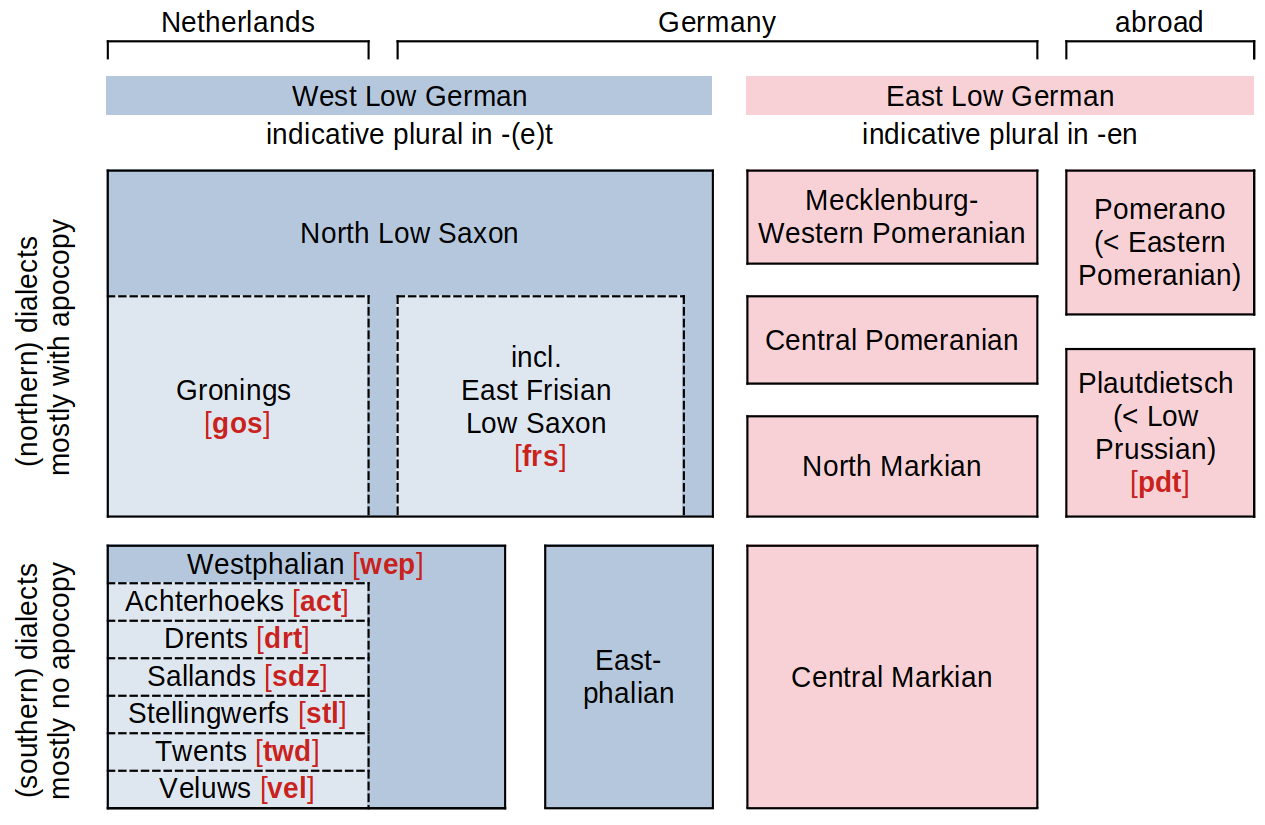
\includegraphics[width=1.0\linewidth]{img/dialects-and-iso632-codes.png}
    \caption{Major dialects of Low German (ISO 639-2 \code{nds}), with regional ISO 639-3 codes in red square brackets.}
    \label{tab-dialects-and-isocodes}
\end{table}

Despite its challenges, Low German enjoys cultural and regional recognition. Efforts to revitalize the language include educational programs, literature, radio broadcasts, and online initiatives. However, without stronger support on many levels, the survival of Low German as a living language remains uncertain. In fact, social networks and digital language resources may play a role in transmission and revitalization of the Low German language, and indeed, this is what we see for other minority languages all over the world. 
To preserve Low German, more work is needed to integrate it into digital spaces. Developing NLP tools, expanding online resources, and increasing its presence in modern media are crucial steps in ensuring that Low German remains a functional and thriving language for future generations. At the moment, however, even the most basic NLP resources are still lacking. For Low German, only small samples of annotated major corpora are known to exist, no parallel corpora (although translated texts can be found, mostly translated into Low German), and no machine-readable dictionaries. 

A \emph{machine-readable dictionary (MRD)} is a structured lexical resource designed for computational use rather than human readability. Unlike traditional dictionaries, MRDs are formatted in a way that allows software applications to process and analyze linguistic data efficiently. They store information such as word meanings, grammatical properties, pronunciations, and translations in a structured manner to facilitate the development of downstream applications. For low-resource languages, \emph{machine-readable dictionaries} (MRDs) play a crucial role in developing foundational NLP technologies. In particular, this is the case for language varieties that have been the subject of linguistic research in the past (so that word lists or dictionaries are available), but that have been largely neglected by NLP or corpus linguistics (so that no digital corpus data is available). This paper addresses the development of an initial set of MRDs for different varieties of Low German. 
Despite being a literary language for about a thousand years and an extant regional literature from the 19th and 20th c., this is the case for Low German: Textual material is available, but not in digital form. Since low resource languages lack large annotated corpora, extensive linguistic databases, or pre-trained models, MRDs serve as a primary data source for computational applications. They facilitate the creation of essential tools such as spell checkers, part-of-speech taggers, and lemmatizers, helping bridge the technological gap between widely spoken and endangered languages. We can build on a number of digital dictionaries in existence, but each pertains to a different variety and all are designed for human consumption, and not for subsequent use in natural language processing. In addition to that, most of these are copyright-protected, either explicitly or by default copyright (if copyright is undeclared). The approach we suggest can, however, be applied to other Low German dictionaries and dialects if copyright can be secured.
    
A key technology for building structured and interoperable MRDs is \emph{OntoLex-Lemon}, an RDF (Resource Description Framework) vocabulary  designed for representing lexical and semantic data on the web. OntoLex allows lexicons to be linked to external knowledge bases and other linguistic resources, enhancing interoperability. It uses, RDF, a W3C standard, to provide a flexible, graph-based data model that enables rich semantic annotations and structured linguistic relationships. Together, these technologies ensure that dictionaries for low-resource languages are not isolated but can be \emph{integrated into broader linguistic ecosystems}, facilitating cross-linguistic research and NLP. By leveraging OntoLex and RDF, MRDs for low-resource languages can be built in a way that supports automated processing, encourages digital preservation, and enables their incorporation into modern NLP applications. These technologies make it easier to link lexical resources across languages, ensuring that low-resource languages gain better representation in computational linguistics and digital tools. As such, OntoLex has been a cornerstone for integrating lexical data into the Linguistic Linked Open Data (LLOD) cloud. 

The \emph{Linguistic Linked Open Data (LLOD)} cloud is a structured network of interlinked linguistic resources published in accordance with the principles of Linked Data \cite{bizer2009linked}. It provides a semantic web-based infrastructure for representing and integrating linguistic data, including lexicons, corpora, terminologies, and ontologies. By leveraging RDF (Resource Description Framework) and related technologies, the LLOD cloud enables interoperability and data exchange across various NLP and linguistic applications \cite{chiarcos2013linguistic}.  A key advantage of the LLOD approach is its ability to connect diverse linguistic datasets, making them accessible for computational use. Resources such as OntoLex-Lemon facilitate the representation of lexicons, while linguistic ontologies like OLiA (Ontologies of Linguistic Annotations) provide standardized annotation frameworks \cite{chiarcos2012olia}. The LLOD cloud benefits low-resource languages by linking their limited linguistic data to richer datasets, fostering NLP development and linguistic research. By structuring linguistic resources using open standards, the LLOD cloud contributes to the creation of multilingual and interoperable NLP systems, supporting tasks such as machine translation, semantic search, and corpus analysis. As the LLOD cloud expands, it plays an increasingly vital role in the digital preservation and computational accessibility of linguistic knowledge.  


%digital and digital-born Low German dictionaries

%Selected digital dictionaries

%\begin{itemize}
%    \item https://woerterbuchnetz.de/?sigle=WWB&lemid=A00001
%    \item Digitales Wörterbuch Niederdeutsch (dwn), https://www.niederdeutsche-literatur.de/dwn/
%    \item https://www.ndr.de/kultur/norddeutsche_sprache/plattdeutsch/woerterbuch101.html: unregulated orthographies
%    \item Plattmakers
 %   \item https://www.platt-wb.de/
  %  \item WöWö
   % \item Mittelelbisches (nur A-O, https://mew.uzi.uni-halle.de/artikel/25748)
    %\item https://www.plattdeutsches-woerterbuch.de/search (suche nach leerem string, um alles zu bekommen), keine einzelseiten
%    \item https://netz.sass-platt.de/hoch-platt
%    \item wiktionary
%\end{itemize}

A number of digital, and in parts, digital-born, dictionaries of different varieties of Low German are available online. As far as Germany is concerned, the only digital Low German dictionary with a permissive license we are aware of is Wiktionary, a collaborative, crowd-sourced dictionary covering multiple languages, including Low German. Includes definitions, pronunciation guides, etymology, and translations. As a crowd-sourced resource, it lacks standardization, as different sets of orthographic conventions are applied by different contributors. Another, digital-born dictionary -- although only available in MS Office and PDF formats -- is Wöhrner Wöör (WöWö), a Low German dictionary for the Dithmarschen variety of North Low Saxon by Peter Neuber, originally published in print in 2001, but subsequently published as PDF and MS Office documents only.\footnote{\url{https://ditschiplatt.de/woehrner-woeoer/}} 
With permission of the author, % WHICH WE DON'T HAVE YET
we use this as the basis for our efforts.

Other digital dictionaries of Low German are available under restrictive (or implicit, i.e., restrictive-by-default) licenses include the following:

\begin{description}
\item[Sass’ Plattdeutsches Wörterbuch] (\href{https://netz.sass-platt.de/hoch-platt}{Sass-Netz})  
    Based on Johann Sass' Plattdeutsch dictionary, which defines a standardized spelling system. Provides High German → Low German translations and is one of the most widely accepted spelling systems for written Plattdeutsch, albeit a deficient one (several sounds are systematically conflated) that also is not applicable to all varieties. In particular, the orthography lacks support for Westphalian, Eastphalian and Central Markian, whereas northern varieties (esp., North Low Saxon) can be represented more or less faithfully. Copying is explicitly restricted to private, non-commercial use. We assume that this also rules out academic usage.

\item[Digitales Wörterbuch Niederdeutsch (DWN)] is a collection of digital Low German dictionaries covering multiple dialects.\footnote{\url{https://www.niederdeutsche-literatur.de/dwn/}} It seems to be developed and maintained by a single individual only, albeit in parts in collaboration with academic partners (e.g., the Kompetenzzentrum für Niederdeutschdidaktik of the University of Greifswald, for whose Mecklenburgian dictionary it provides the technical backbone).\footnote{\url{https://länderzentrum-für-niederdeutsch.de/renate-hermann-winter-woerterbuch-nun-online/}} The dictionaries are searchable and provide semi-structured HTML content. No explicit license is given, thus restricted copyright. It should be noted, however, that the original copyright of several dictionaries provided via DWN has expired. Yet, database right applies to the digital edition. Aside from an all-over Low German dictionary compiled from diverse sources, it also provides regional dictionaries.

\item[Westfälisches Wörterbuch (WWB)] is a comprehensive academic dictionary of Westphalian, as spoken in northwestern Germany, made available as part of the Wörterbuchnetz platform \cite{wwb}.\footnote{\url{https://woerterbuchnetz.de/}}. It provides detailed historical and etymological information in semi-structured HTML. The Wörterbuchnetz also provides an API access, although only to lemma lists and full text search, not to the actual entries. No explicit license is given, thus restricted copyright.

\item[NDR Plattdeutsch Wörterbuch] aims to be a general Low German dictionary and is hosted by Norddeutscher Rundfunk (NDR).\footnote{\url{https://www.ndr.de/kultur/norddeutsche_sprache/plattdeutsch/woerterbuch101.html}} Most of its content seems to be crowd-sourced, it thus contains unregulated orthographies, so that words appear in varying spellings or for different dialects. Focuses on practical and everyday vocabulary rather than linguistic precision. No explicit license is given, thus restricted copyright.

\item[Plattmakers] \href{https://plattmakers.de} is a collaborative online Low German dictionary, similar to Wiktionary, based on a digital-born multi-dialectal core dictionary developed by Marcus Buck in 2009. It covers all Low German dialects, providing translations in German, Dutch, and English. Lemmas are normally given in North Low Saxon or normalized to a North Low Saxon pronounciation. Words include regional maps, explanations in Low German, and cognates in High German, English and Dutch. Without an explicit license statement, the content is copyright-protected.

\item[Online-Wörterbuch für ostfriesisches Plattdeutsch] (\href{https://www.platt-wb.de/}) 
    is a dictionary portal that provides search over a dictionary for East Frisian Low German, compiled from various sources and edited by the Plattdüütskbüro der Ostfriesischen Landschaft. The dictionary is free searchable for German and Low German in both directions, and support partial matches. Without explicit license statement, it is copyright-restricted.

\item[Mittelelbisches Wörterbuch] (\href{https://mew.uzi.uni-halle.de/artikel/25748}{MEW})
    A dictionary of Middle Elbe Low German, currently covering only A–O. Subject of an ongoing linguistic research project based at the University of Halle.  The dictionary is published under CC BY-NC-ND. We interpret the ND clause as prohibiting the conversion to a Linked Data representation.

\item[Platt för Plietsche; Plattdeutsch Übersetzer für Schleswig-Holstein, Hamburg, Bremen und Teilbereiche von Mecklenburg-Vorpommern und Niedersachsen] (\href{https://www.plattdeutsches-woerterbuch.de/}) provides search over a bilingual German-Low-German word list. Without explicit license statement, this is copyright-protected.



\end{description}

Major dictionaries available in print (or PDF) only include the Berlin-Brandenburg dictionary, the Niedersächsisches Wörterbuch, the Pommersches Wörterbuch, the Schleswig-Holsteinisches Wörterbuch \cite{mensingotto}. The Wossidlo-Teuchert dictionary of Mecklenburgian is currently in the process of integration into Wörterbuchnetz.\footnote{\url{https://www.germanistik.uni-rostock.de/personen/professuren/prof-dr-andreas-bieberstedt/projekte-und-forschungsschwerpunkte/wossidlo-teuchert-online/}}

More dictionaries:
- Das Niedersächsische Wörterbuch ist bislang ebenfalls nur in print verfügbar und nur bis zum buchstaben s veröffentlicht, vgl. https://www.uni-goettingen.de/de/publikationen/219293.html



As for machine-readable dictionaries of Low German, we are not aware of any Low German lexical datasets except for Low German terms in foreign-language editions of DBnary, i.a., the database edition of the Wiktionary, also cf. ACoLi dictionary graphs. However, PanDoc data is generally of mixed quality, as it is largely based on automated OCR. Wiktionary data is crowdsourced, and for a language without a written standard, this data is too unsystematic to be used and reliably linked with other lexical resources, as it freely mixes mixes regional and author-specific orthographies.

In addition to these dictionaries, there are many print dictionaries, also in the public domain, but not reliably digitized.

\section{Wöhrner Wöör (WöWö)}

\subsection{Overview and Digital Evolution}

The \emph{Wöhrner Wöör} is a Low German dictionary from the Dithmarschen region (North Low Saxon), compiled by Peter Neuber (born 1939 in Stettin), a linguist and educator. The dictionary was created with the goal of documenting and preserving the traditional vocabulary and expressions of Plattdeutsch while simultaneously adapting the language to modern contexts. Beyond recording historical terms, Neuber sought to introduce neologisms for contemporary concepts that previously lacked Low German equivalents, integrating them into the lexicon.

First published in 2001 in Wöhrden, the \emph{Wöhrner Wöör} consists of 699 pages and serves as a German-to-Low-German reference work specific to the Dithmarschen dialect. Following its initial print release, the dictionary has undergone continuous expansion, with subsequent versions distributed exclusively in digital formats such as Microsoft Word and PDF. Within the \emph{Niederdeutsche Literaturdatenbank} (Low German Literature Database), the 2017 Word edition is the most frequently cited version. The latest version, titled \emph{Ditschiplatt: Wöhrner Wöör} from January 2019 is online accessible.\footnote{\url{https://ditschiplatt.de/woehrner-woeoer/}}

A major structural update took place at the end of 2015, when Neuber transitioned the dictionary's orthography to an extended version of the SASS spelling system, originally developed by Johannes Sass. This modified system incorporates diacritical marks (macrons) to denote diphthongs, thereby enhancing phonological precision. Beyond its lexical entries, the dictionary includes a comprehensive user guide for navigating the digital version in MS Office (Word), as well as pronunciation information and a grammatical overview of the Dithmarschen dialect, with a particular focus on verbs, nouns, and adjectives.

Despite its detailed documentation and modern adaptation efforts, the \emph{Wöhrner Wöör} remains primarily a resource for human readers, lacking structured machine-readable representations that would facilitate its use in NLP applications. Thus, our goal was to convert the \emph{Wöhrner Wöör} into an RDF-based format following the OntoLex-Lemon model to ensure interoperability with other lexical datasets and enable the dictionary’s inclusion in the Linguistic Linked Open Data (LLOD) cloud, paving the way for broader computational applications and cross-linguistic research.

\begin{figure}
    \centering
    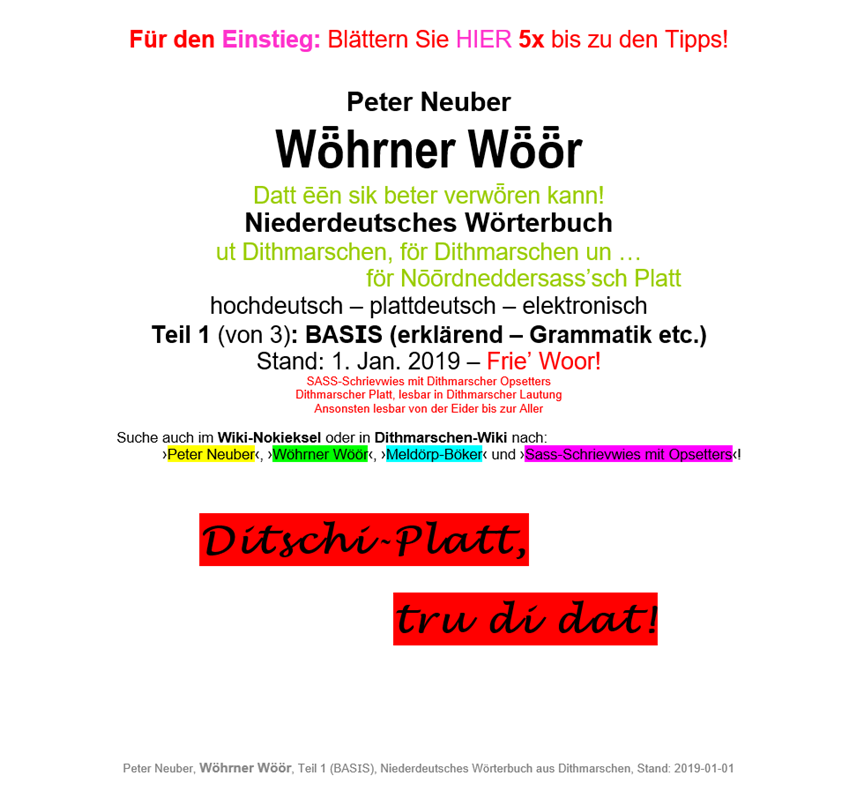
\includegraphics[width=1\linewidth]{img/woewoe_cover.png}
    \caption{Front page of the \emph{Wöörner Wöhr} dictionary in docx format.}
    \label{fig:enter-label}
\end{figure}

\begin{figure}
    \centering
    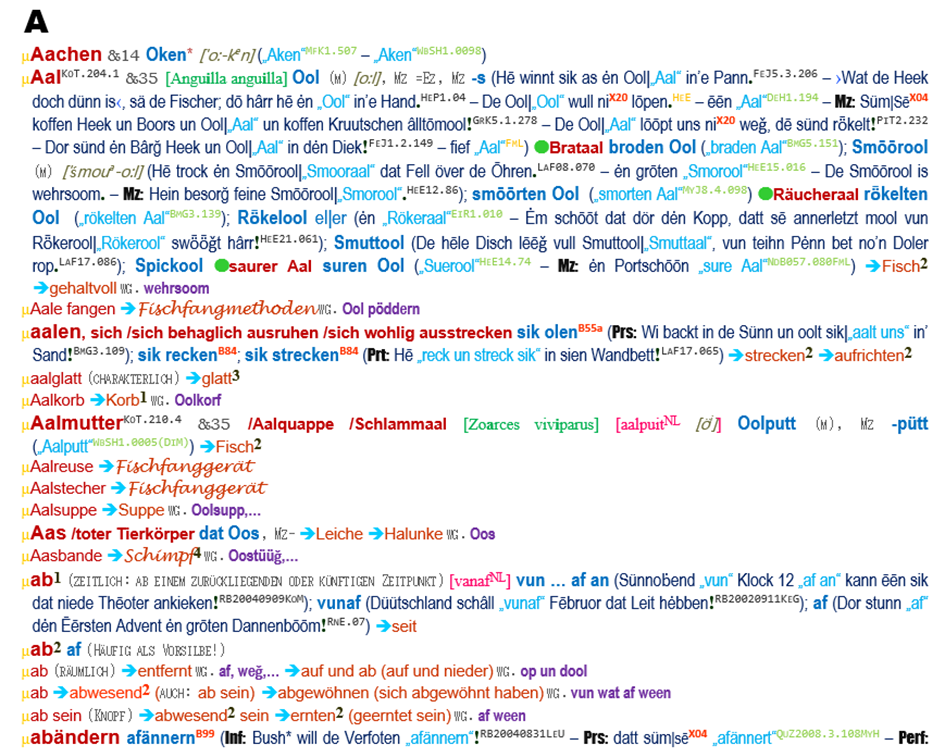
\includegraphics[width=1\linewidth]{img/woewoe_excerpt.png}
    \caption{Excerpt of the first entries under ‘A’ from the beginning of the lexical part of the \emph{Wöörner Wöhr} dictionary in docx format.}
    \label{fig:enter-label}
\end{figure}

\subsection{Converting the WöWö}

Converting the \emph{Wöhrner Wöör} into a \emph{machine readable dictionary} (MRD) posed a significant challenge due to its highly fragmented docx format. The extensive use of diverse fonts, colors, and sizes—each encoding different functions—meant that the underlying text information was split into numerous small fragments within the xml format. This complexity required a multi-stage processing pipeline via Python for extraction, merging, and transformation of the text information:

\begin{enumerate}
    \item \textsf{\textbf{XML Extraction and Initial CSV Creation}}\\  
    First, the underlying XML structure of the Word document is parsed using Python’s \texttt{xml.etree.ElementTree}. Each text run (\texttt{<w:r>}) is extracted along with its formatting metadata (font, color, and size), leveraging XML namespaces to accurately retrieve \texttt{<w:t>} (text) and \texttt{<w:rPr>} (formatting) elements. This step generates a preliminary DataFrame, which is then exported as a CSV file.

    \item \textsf{\textbf{Merging Consecutive Text Blocks}}\\  
    Due to fragmentation, consecutive text blocks that share the same formatting should be merged. A Python script iterates over the DataFrame and combines text segments when the formatting—specifically color and size—remains unchanged. This merging produces a more coherent CSV that better reflects the original document’s logical groupings.

    \item \textsf{\textbf{Structuring the Data into a Lexical CSV}}\\  
    With the merged text available, the next step involves classifying and extracting entries into five columns, depending on the corresponding formatting:
    \begin{enumerate}
        \item {\textbf{High German Main Lemma}}
        \item {\textbf{High German Sublemma}}\\Potentially existing subentries for the lexical entry.
        \item {\textbf{Low German Translation}}
        \item {\textbf{Low German Additional Information}}\\ Additional grammatical information—mainly plural forms—that has the same formatting as the corresponding Low German lexical entry.
        \item {\textbf{Low German IPA Information}}\\Available Low German phonetic transcriptions.
    \end{enumerate}
    This structured CSV serves as the foundation for converting the data into RDF.

    \item {\textbf{Generating RDF (Turtle Format)}}\\ 
    Separate Python scripts convert the structured CSV data into RDF using the Turtle syntax:
    \begin{enumerate}
        \item {\textbf{High German Entries:}} Entries are first grouped by main lemmas. The script converts them into \texttt{ontolex:LexicalEntry} nodes, each with its own lexical sense (\texttt{ontolex:LexicalSense}). Additional information, such as synonymous terms or usage examples—but mostly plural information or alternative spellings (e.g., variations in single vowels)—is included as \texttt{ontolex:otherForm}. In the case of alternative spellings or plural information, these additions are usually not full words but only the modifications, such as the suffix '-s'. A custom property (\texttt{neuber:subEntry}) links related sublemmas. For all existing sublemmas, individual lexical entries with their own lexical senses are generated in a similar way.
        \item {\textbf{Low German Translations:}} The Low German translations are processed into lexical entries, each with its own lexical sense. If available, IPA notation is incorporated into the canonical form as \texttt{ontolex:phoneticRep}.
        \item {\textbf{Linking Translations:}} Finally, unique \texttt{vartrans:translation} entries are generated to link source senses (from main or sublemma entries) with their corresponding target senses (translations).
    \end{enumerate}

    \item {\textbf{Post-Processing}}\\  
    The generated Turtle files are further refined using a regex-based clean-up. This post-processing step removes unnecessary whitespaces, replaces dashes with underscores, and normalizes punctuation to ensure that the RDF output adheres to the required naming conventions and syntactic standards.
\end{enumerate}

This comprehensive pipeline successfully transforms the fragmented docx format of the \emph{Wöhrner Wöör} into a coherent RDF dataset, aligning the dictionary with the Ontolex-Lemon model. [Making it possible to integrate it into the Linguistic Linked Open Data (LLOD) ecosystem?]. So far, this extraction process has focused on retrieving the most essential information—lexical entries, written and phonetic representations, and their corresponding translations. However, the \emph{Wöhrner Wöör} contains numerous additional details for each entry, such as references and usage examples, which are more challenging to extract due to the complexity of the fragmented formatting.

\begin{figure}
    \centering
    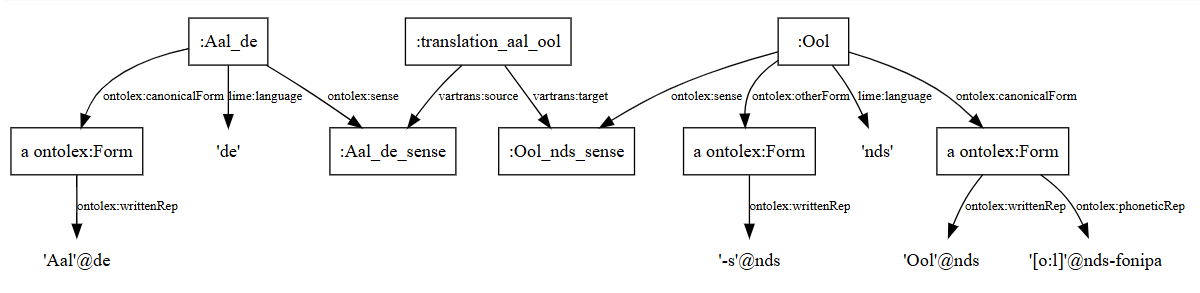
\includegraphics[width=1\linewidth]{aal-rdf-graph.png}
    \caption{Enter Caption}
    \label{fig:enter-label}
\end{figure}

%digraph finite_state_machine {
%    rankdir=UD;
%    size="8,5"
%    node [shape=box, fontname="CMU Serif"];
%        edge [fontname="CMU Serif", fontsize=11];
%
%        Aal [label=":Aal_de"];
%        Aal_canonicalForm [label="a ontolex:Form"];
%        Aal_sense [label=":Aal_de_sense"];
%        translation_aal_ool [label=":translation_aal_ool"];
%        Ool [label=":Ool"];
%        Ool_canonicalForm [label="a ontolex:Form"];
%        Ool_sense [label=":Ool_nds_sense"];
%        Ool_otherForm [label="a ontolex:Form"];
%
%        Aal -> "'de'" [label = "lime:language"];
%        Aal -> Aal_canonicalForm [label = "ontolex:canonicalForm"];
%        Aal -> Aal_sense [label = "ontolex:sense"];
%        translation_aal_ool -> Aal_sense [label = "vartrans:source"];
%        translation_aal_ool -> Ool_sense [label = "vartrans:target"];
%        Ool -> Ool_canonicalForm [label = "ontolex:canonicalForm"];
%        Ool -> Ool_sense [label = "ontolex:sense"];
%        Ool -> Ool_otherForm [label = "ontolex:otherForm"];
%        Ool -> "'nds'" [label = "lime:language"];
%        Aal_canonicalForm -> "'Aal'@de" [label = "ontolex:writtenRep"];
%        Ool_canonicalForm -> "'Ool'@nds" [label = "ontolex:writtenRep"];
%        Ool_canonicalForm -> "'[o:l]'@nds-fonipa" [label = "ontolex:phoneticRep"];
%        Ool_otherForm -> "'-s'@nds" [label = "ontolex:writtenRep"];
%
%        "'de'" [shape=none];
%        "'nds'" [shape=none];
%        "'Aal'@de" [shape=none];
%        "'Ool'@nds" [shape=none];
%        "'-s'@nds" [shape=none];
%        "'[o:l]'@nds-fonipa" [shape=none];
%}

\section{Linking the WöWö}

A number of online dictionaries for Low German are available, but usually not under permissive licenses. As a result, we focus on the WöWö dictionary as our primary dataset, and do currently not provide Linked Data editions of other Low German dictionaries. However, these are accessible online, usually with URIs identifying the respective lemma, and we use only \emph{this information} (the existence of a lemma and the assignment of a particular URL) to create an index for these in RDF. We neither apply nor use any specific information from the dictionaries other than the existence of a lemma, we assume that this information does not meet the threshold of originality legally required for copyright to apply,\footnote{See \citet{Margoni2016} for the threshold of originality in EU copyright law.}
so that these LOD indices to other Low German dictionaries can be published as addenda to the WöWö dataset regardless of the licensing situation of the full data sets. However, should these respective resources be ever served as Linked Data or be made accessible under a more permissive license, the information from the indices/links we provide can be seamlessly integrated into the respective dictionaries.

At the moment, however, any of the dictionaries we are going to work with are perfect silos, in the sense that they are isolated from any other content available on the web. Yet, this does not mean that they do not contain links. In fact, \emph{several} of the existing platforms have been \emph{designed} to provide inter-dialectal links, resp., links between different dictionaries, but they only provide links \emph{within} the respective ecosystem, whereas we pursue an open, extensible approach capable of integrating \emph{any} piece of information accessible on the web. 

\begin{itemize}
\item The Trier Wörterbuchnetz\footnote{\url{https://woerterbuchnetz.de/}} is an online platform that provides access to a wide range of dictionaries of historical and regional vernaculars from Germany, including dictionaries for historical stages and dialects of German and related varieties, but also dictionaries of Latin, Ladin, Uighur and Russian. In addition, it comprises a major dictionary of the Westphalian dialect of Low German. Aside from basic search, it provides links between languages of related varieties. This includes bibliographical references, but also HTML hyperlinks. Overall, the Wörterbuchnetz builds on a mature stack of XML technologies established during the past two decades. The platform and its content are freely accessible online, and in addition to the human-readable content, there also exists an API that can be used to retrieve lists of lemmata and their attestations. The content itself, however, is not provided in a machine-readable form. Within the Wörterbuchnetz, however, hyperlinks are limited to resources provided by the Wörterbuchnetz itself. It is thus not possible to perform inter-dialectal search for different varieties of Low German within that platform directly. This might change with a project targeted towards integrating major Low German dictionaries into the Wörterbuchnetz currently pursued at the University of Rostock, Germany, but then, again, the existing Wörterbuchnetz technology will only be able to provide links between these resources, but not between them and other dictionaries.
\item The Digitales Wörterbuch Niederdeutsch (DWN)\footnote{\url{https://www.niederdeutsche-literatur.de/dwn/}} by Peter Hansen is a website that provides access to a `basis' Low German dictionary (adopting spelling rules developed for North Low Saxon), a dictionary for Mecklenburgian-Western Pomeranian as well as custom dictionaries for major authors (Klaus Groth, Fritz Reuter and John-Brinckman Wörterbuch). Each dictionary comes with its own search dialog, and little is known about the technical details, as only a human-readable HTML rendering is accessible. Within each dictionary, lemmata are linked across these datasets with HTML links. We presume that this uses standard SQL technology. Again, no links to external resources are being provided.
As the content is copyright-protected, we decided to work only with one of these dictionaries \citep{muller1904reuter}, whose content actually goes back to a print dictionary in the public domain. So, we did not exploit the interdialectal links provided by the DWN, nor did we use any of its original content.
\item Plattmakers\footnote{
    \url{https://plattmakers.de/de}
} is an online aggregate dictionary with 22.000 entries provided in a single, searchable database, and developed by Marcus Buck. It provides its content in human-readable fashion, and individual entries are equipped with maps and links to the source literature. Plattmakers is a private website, but some details about its implementation are provided,\footnote{\url{https://plattmakers.de/de/faq}} indicating that it is based on a relational database backend, and supported by automated normalization routines similar to those described below. Unlike DWN and Wörterbuchnetz, Plattmakers lemma URLs provide machine-readable metadata in JSON-LD, so that its content \emph{can} be processed and evaluated in conjunction with WöWö information. At the same time, it is copyright-protected, so that we do not work with any Plattmakers information except for URL and lemma form. Unlike DWN and Wörterbuchnetz, Plattmakers is a private initiative not supported by any academic institution, and some of its more recent content seem to be crowd-sourced and not to meet scientific standards. Yet, it is seems to be more usable than either DWN or Wörterbuchnetz, because it provides direct, interdialectal search capabilities across all dictionaries it covers. We assume that our linking implementation partially replicates functionalities that have been developed in the Plattmakers backend before, but that we provide an added value in extending these to content not covered by Plattmakers, and in particular, to other dictionaries maintained by academic providers, so that conjoint queries over WöWö, Plattmakers, DWN and Wörterbuchnetz information are capable of providing more detailed (and, in parts, better substantiated) information than queries over Plattmakers content alone.
\end{itemize}

Overall, six online dictionary have been linked with the WöWö, with lexical sources covering the main branches of modern Low German:

\begin{itemize}
\item For North Low Saxon, we link the Plattmakers dictionary. (WöWö is North Low Saxon, as well, and Plattmakers actually includes other dialects, but normalizes to North Low Saxon orthography.)
\item For Westphalian (in German orthography), we link the Wörterbuchnetz Westphalian dictionary.
\item For Dutch Low German dialects, we link the Twents Woordenboek by Goaitsen van der Vliet (2025), available for online search under \url{https://twentswoordenboek.nl} and published under CC BY-NC-SA. Twents is another Westphalian dialect.
\item For East Low German (in Germany), we use DWN Reuter dictionary, which represents Mecklenburgian-Western Pomeranian dialect.
\item For emmigrant varieties of East Low German, we work with a Plautdietsch (Mennonite Low German) dictionary developed by Herman Rempel and the Mennonite Literary Society (1984-1995), \url{mennolink.org} (1998-2006), and Eugene Reimer (2006-2007). The data is available as a plain HTML file under CC BY-SA.\footnote{\url{https://ereimer.net/plautdietsch/pddefns.htm}}
\end{itemize}

This data is relatively diverse in phonology and orthography, so that formal linking must not rely on mere identity. Instead, we use Finite State Transducers to generate hypothetical normalizations against one specific variety of Low German and then generate candidate links for lemmas from different dictionaries for which identical forms are generated (see Sect. \ref{sec-linking-by-agreement}).

\subsection{Data Retrieval and Processing}

Creating an LOD index for a dictionary (portal) typically requires to retrieve (crawl) its complete content, to extract lemma forms and lemma URL and to store these in a TSV file. Optionally, additional information (parts of speech, translation/definition, etc.) can be included in additional columns. For these initial TSV files, we then create an extended TSV file that adds two additional columns, the lemma form in WöWö (for verification), and the WöWö URL (for the actual linking). At the dictionaries that WöWö will be linked with comprise form-level information, only, linking is grounded on \emph{formal agreement} only (see below), so that in most cases, there are many-to-many relationships between dictionary lemmas and WöWö entries (cf. Fig. \ref{fig-twents-woewoe}).

\begin{figure}
    \centering
    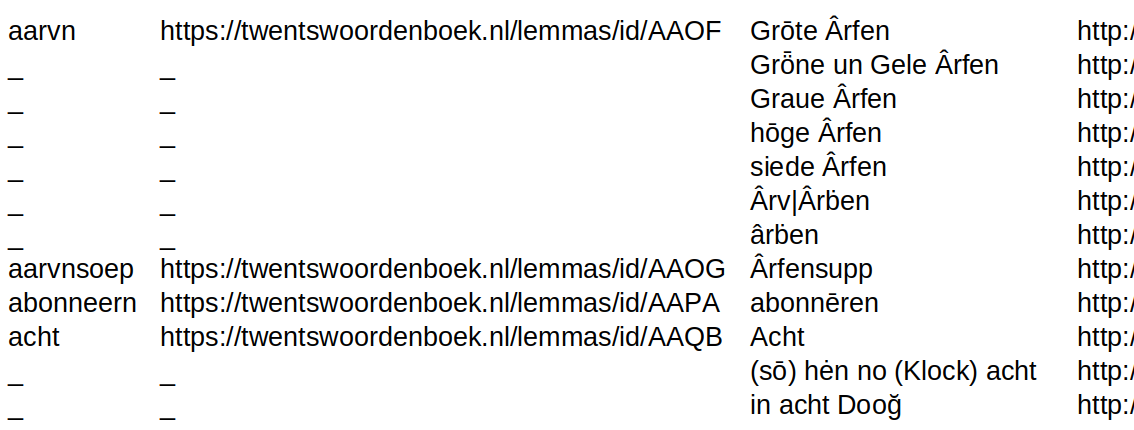
\includegraphics[width=1.0\linewidth]{img/tsv-linked.png}
    \caption{Linked TSV file except, Twents (left) to WöWö (right)}
    \label{fig-twents-woewoe}
\end{figure}

For the RDF export, we calculate the confidence of a link $\langle x,y\rangle$ as the harmonic mean between the linking probabilities $P(x|y)$ and $P(y|x)$, with $P(x|y)$ and $P(y|x)$  estimated from the many-to-many relationships from the extended TSV file. In the RDF export, we only include the most probable links. If there is more than one, we return the WöWö lemma with the lowest Levenshtein distance. If there is still more than one, we return the shortest WöWö lemma. If there is still more than one, we return the lexicographical first lemma.\footnote{
    The converter has a flag to return all possible links, along with their confidence, but this is disabled by default.
}

\subsection{RDF Representation}

Although, optionally, all links can be returned, the RDF export only contains the most confident link, by default. For any given link $\langle x,y\rangle$, the confidence score $c(x,y)$ is calculated as $c(x,y)=2 \frac{P(x|y) P(y|x)}{P(x|y) + P(y|x)}$. If more than one match with the same score is found, we return the one with lowest Levenshtein distance. If this is not umambiguous, we return the shortest target URL in order to create a bias against matches between multi-word expressions and their respective parts.

For every external dictionary, we create one lexical entry per source URL, and provide the lemma form as its canonical form. These lexical entries are then linked with WöWö URLs.

We produce linking files in two different flavours. The condensed format only conveys a \onto{lexinfo:geographicalVariant} link between two lexical entries.\footnote{
    `Geographical variant' is not a perfect term to describe the cross-dialectal relation between individual lexical entries, because this implies that both variants are, in fact, different. However, in many cases they are not, or their differences are merely orthographic. Better suited would be a relation that can be applied to lexical entries that are either equivalent, (virtually) identical or deviant. 
    Although more appealing from its name, we decided to not resort to \onto{lexinfo:approximate}, because it's a sense relation, not a relation induced by forms ... the sense link is unconfirmed and we don't have machine-readable senses for any dictionary other than WöWö.
}
This compact format is well-suited for downstream applications where only the link itself is processed, but it omits provenance and confidence information. Unlike the reified export described below, this is also OWL2/DL-compliant. 

As there is no manual quality control involved here and the automated linking procedure creates many n:m correspondences, it is, however, preferred to provide the confidence scores, as well, for which we adopt a reified representation inspired by \citet{gillis2023refinement}, with a \code{vartrans:LexicalRelation} object that \code{vartrans:relates} an external lexical entry with a lexical entry from WöWö and that uses \code{lexinfo:category} to indicate the type the of relation. There are, however, no exactly corresponding concepts in lexinfo to indicate the type of relation, so that, instead of an individual, we resort to \onto{lexinfo:geographicalVariant}, again. However, this is an object property, not an individual, the resulting data is thus propelled into the semantic space of OWL2/Full.

Every reified link is complemented with a numerical confidence score. Due to the lack of a standard vocabulary for confidence scores in RDF or LexInfo, we adopt \onto{rdf:value} for the purpose, but this is semantically underspecified. We would recommend to create a designated LexInfo property, say, \onto{lexinfo:confidence}.

For the example of WöWö \word{Ool} and its cognates in the Twente dictionary, we arrive at the graph in Fig.\ \ref{fig-links}. The lexical entry \onto{:Ool} is the entry from the RDF edition of WöWö, the individual links are formally associated with a dataset object, like the individual dictionary entries are associated with their source URL that is defined as a \onto{lime:Lexicon}. However, as we only provide a shallow wrapper around the original source document, and because the URLs will not resolve to machine-readable information, we bundle both linking information and the lexical entries drawn from \url{https://twentswoordenboek.nl} in a single file.

\begin{figure}
    \centering
    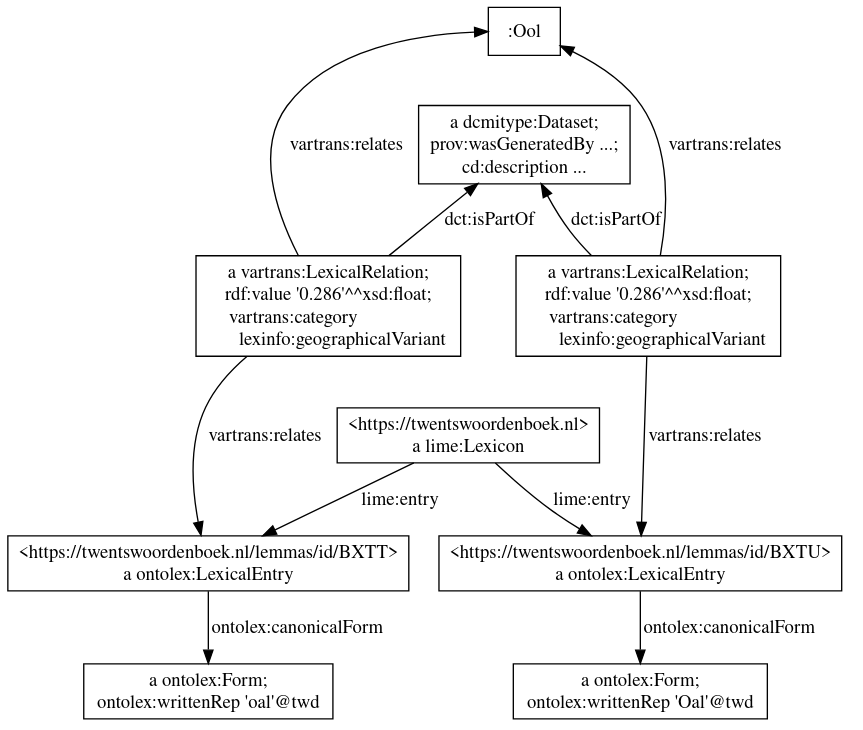
\includegraphics[width=0.9\linewidth]{img/links-vis.png}
    \caption{Reified \onto{lexinfo:geographicalVariant} links between WöWö \word{Ool} `eal' and Twents dictionary}
    \label{fig-links}
\end{figure}

%% Dot source
% digraph G {
% 
%  ool -> bxtt_link [label=" vartrans:relates", dir=back]
%  ool -> bxtu_link [label=" vartrans:relates", dir=back]
%  ool -> ds[style=invis]
%  ool [label=":Ool",shape=box]
% 
%  ds -> bxtt_link[dir=back, label="dct:isPartOf"]
%  ds -> bxtu_link[dir=back, label="dct:isPartOf"]
% ds[label="a dcmitype:Dataset;\nprov:wasGeneratedBy ...;\ncd:description ...", shape=box]
% 
% twents[label="<https://twentswoordenboek.nl>\n a lime:Lexicon", shape=box]
% twents->bxtt[label="lime:entry"]
% twents->bxtu[label="lime:entry"]
% 
%  bxtt_link[label="a vartrans:LexicalRelation; \nrdf:value '0.286'^^xsd:float;\nvartrans:category               \n       lexinfo:geographicalVariant", shape=box]
%  bxtu_link[label="a vartrans:LexicalRelation; \nrdf:value '0.286'^^xsd:float;\nvartrans:category               \n       lexinfo:geographicalVariant", shape=box]
% 
% bxtt_link->twents[style=invis]
% 
%  bxtt_link ->  bxtt [label=" vartrans:relates",constrains=false]
%  bxtu_link ->  bxtu [label=" vartrans:relates"]
% 
%  bxtt -> oal_twd [label=" ontolex:canonicalForm"]
%  bxtt [label="<https://twentswoordenboek.nl/lemmas/id/BXTT>\n a ontolex:LexicalEntry", shape=box]
%  oal_twd [label="a ontolex:Form;\nontolex:writtenRep 'oal'@twd", shape=box]
% 
%  bxtu -> Oal_twd [label=" ontolex:canonicalForm"]
%  bxtu [label="<https://twentswoordenboek.nl/lemmas/id/BXTU>\n a ontolex:LexicalEntry", shape=box]
%  Oal_twd [label="a ontolex:Form;\nontolex:writtenRep 'Oal'@twd", shape=box]
% 
% }

Another apparent gap in LexInfo is the lack of a counterpart of translation set for lexico-semantic relations other than translation. In its place, we resort to \url{http://purl.org/dc/dcmitype/Dataset}. This is needed to store provenance information (which otherwise needs to be repeated for every lexical link). Every lexical-semantic relation is linked by \onto{dct:isPartOf}.

\subsection{Language Identification}

We provide fine-grained, dialect-level language tags for the different varieties. For this purpose, we use the most fine-grained ISO 639-3 language identifier applicable (or, if no dialect-specific ISO 639-3 language tag is defined, we resort to the language tag \code{nds} as understood in ISO 639-2).\footnote{
    The language tag \code{nds} is also included in ISO 639-3 for `Low German / Low Saxon', but its scope in ISO 639-3 is uncertain, as a number of Low German dialects (but not all) are assigned individual language tags, but the remaining `\code{nds}' dialects do not correspond to a linguistically well-defined dialect group.
} 
% for dialect identification we use https://de.wikipedia.org/wiki/Schleswigsch#/media/Datei:Verbreitungsgebiet_der_heutigen_niederdeutschen_Mundarten-2.PNG
Where applicable, these language tags are combined with Glottolog identifiers,\footnote{\url{https://glottolog.org}} marked as a private-use subtag (i.e., separated by \code{-x-}) in accordance with BCP47.\footnote{\url{https://www.rfc-editor.org/info/bcp47}}, so we use 
\code{nds-x-dith1234} (Dithmarsh) for WöWö,
\code{nds-x-nort3307} (North Hanoveranian) for Plattmakers,
\code{nds-x-hols1234} (Holsteinian) for Sass,\footnote{
    Sass aims to be a multidilectal dictionaries, but their spelling conventions originate from the work of Johann Hinrich Fehrs, a speaker of Holsteinian North Low Saxon
}
\code{nds-x-meck1239} (Mecklenburg-Western Pomeranian) for Reuter,
\code{wep} for the Westphalian dictionary,
    %, we use the unmodified ISO 639-3 tag `wep`, because it uses an artificial, scientific spelling that aims to capture cross-dialectal differences within Westphalian.
\code{twt} for Twents, and
\code{pdt} for Plautdietsch.

Despite the dialect identification, we would like to point out that not all lexemes included in Plattmakers and Sass actually originate from that region and may not even be attested there. Here, the language tag only indicates the spelling conventions adopted in accordance with those of a specific variety.

\section{Linking by Formal Agreement}
\label{sec-linking-by-agreement}

There is no standard orthography for Modern Low German, and the existing dialects differ in their phonology, and, in parts, in their grammar, as well.
In general, North Low Saxon, Mecklenburgian, Pomeranian and North Markian varieties in Germany are written with slightly defective orthographies based on High German. These are defective in the sense that certain phonological differences are not systematically represented. In particular, this pertains to the three-fold differentiation between long (/e:/,/o:/,/ø:/, etc.), lengthened (/ɛ:/, /ɔ:/, /œ:/) and short vowels (/ɛ/, /ɔ/, /œ/) whose writing cannot be directly grounded on High German spelling conventions designed to express the two-fold distinction between long (/e:/,/o:/,/ø:/) and short vowels (/ɛ/, /ɔ/, /œ/), only. 
To address this shortcoming, Plattmakers provides phonological representations for many of its entries. As for the Westphalian dialects in Germany, these are phonologically much richer, so that mostly custom orthographies have been developed. The Wörterbuchnetz orthography uses a scientific notation for somewhat artificially reconstructed interdialectal forms. The orthography of the Twents dictionary is based on the spelling of Dutch. Plautdietsch is written with an independently developed orthography based on influences from English and German spelling.

As a result, lemmas are not easily mappable across the dictionaries. However, historical phonology and the characteristics of the respective orthographies are well understood.
We thus use the Stuttgart Finite State Transducer (SFST) library to normalize the spelling of each specific source to a phonological representation of a specific reference dialect, and for any pair of lemmas that share a reconstructed form in this variety, we predict a possible link. 
As reference dialect, we work with North Markian, an East Low German dialect spoken in the federal states of Brandenburg and Saxony-Anhalt and characterized by its comparably simple phonology: Whereas some Low German dialects distinguish up to 3 different phonemes representing each of the Middle Low German /ê/, /ô/ and the umlaut of /ô/ with different qualities of diphthongs, these are equally realized as monophthongs in North Markian as documented by \cite{pfaff1898vocale}, \cite{mackel1905mundart} and \cite{teuchert1907mundart}. This reduced phoneme inventory also corresponds roughly to some North Low Saxon dialects, including the reference pronounciation and spelling adopted by Plattmakers and the WöWö phoneme inventory.

On the phonological level, Low German dialects differ primarily in their vowel system, and this includes the following processes:

\begin{itemize}
\item diphthongization of long vowels: As an example, we find Reuter \word{Kauken} (WöWö \word{Kōken}) `cake', normalized to \code{kOken}, with \code{O} representing North Markian /o:/. Compare this with Reuter \word{Bom} (WöWö \word{bōōm}) `tree', normalized to \code{bOm}.
\item lengthening and shortening (in all dialects, but in different regions with different results)
\item apocope and syncope: esp. in Northern dialects, unvoiced Middle Low German short vowels have been lost. North Markian is very systematic in the application of apocope and syncope.\footnote{
    There have been approaches to provide an orthographic normalization towards dialects without apocope (esp. \url{https://skryvwyse.eu}), but computationally speaking, the random insertion of vowels into dialect forms with apocope and syncope is less tractable than the deletions of vowels from dialects without.
}
\item other contextual assimilations, e.g., before r, so we find \word{Barg} (Reuter, Twents, Plattmakers 
/baɐç/), 
% /b\overarc{aɐ}ç/), % compiler timeout
along with \word{bearg} (Twents), \word{Boªrg} (Westphalian) and \word{Boajch} (Plautdietsch),  `mountain', normalized to \code{berg}. From Low Prussian, Plautdietsch inherited the contextual lowering of short vowels, so that we find \word{au} /ɔ:/ in place of \word{e} (\word{Aulfenbeen} `ivory', cf. High German \word{Elfenbein}), \word{e} in place of \word{i} (\word{jlebbrijch} `slippy', WöWö \word{glibberig}), etc.
\end{itemize}

Another set of regional differences pertains to /s/ and /ʃ/:

\begin{itemize}
    \item /sk/ $\sim$ /ʃ/: We find Westphalian \word{wisken} `to wish' along with WöWö \word{wischen}, normalized to \code{S} for North Markian /ʃ/.
    \item /s/ $\sim$ /ʃ/ before vowels: We find Plautdietsch \word{schlape} `to sleep' along with WöWö \word{slopen}, normalized to \code{S} for North Markian /ʃ/.
    \item /ʃ/ $\sim$ [ʒ]: In loan words, most Low German varieties normalize foreign /ʒ/ to /ʃ/. Under Slavic influence, /ʒ/ was established as independent phoneme in Plautdietsch, thus Plautdietsch \word{rüzhe} `the sound of water falling' alongside WöWö \word{ruuschen}, normalized to \code{S} for North Markian /ʃ/.
    \item /s/ $\sim$ [z]: For most Low German dialects, voiced [z] is an allophone of /s/ and thus not distinguished in orthography. In Dutch-based orthography, it is nevertheless orthographically distinguished, hence Twents \word{zitte} `manner' alongside WöWö \word{Sitt}. Normalized to /s/.
\end{itemize}

In the FST, we first provide a mapping from source graphemes to North Markian phonemes, represented by a simplified phonological representation using ASCII characters. Where a source language grapheme has different possible readings (or different phonological mappings to North Markian), all possible interpretations are predicted. This also includes a rule to drop \word{e} in all positions. In addition to context-free mappings, this also includes selected contextual assimilations. In addition to the processes mentioned above, this also includes the treatment of final \word{-en}, which is simplified to \word{-e} in Plautdietsch. In a subsequent step, invalid candidate representations are filtered out. For example, the Plautdietsch trigram \word{jch} must be represented as (palatal) \code{x} [ç], not as the sequence \code{jx} (for /j/ with velar /x/).

In general, the mapping generalizes relatively well, but it overgenerates to some extent. As a counter-measure, we calculate confidence scores, and, although also links with low confidence scores are returned, we would in general consider links with confidence scores larger than 0.5 as safe candidates, as this indicates that the mapping is unique in one direction and no more than two alternatives exist for the other direction, see Tab. \ref{tab-results} for statistics.\todo{add Sass to tab-results}



\begin{table}
{\small
\begin{tabular}{ccccc}
                & $c=1.0$   & $c\geq 0.65$  & $c \geq 0.5$  & total \\ \hline
Plautdietsch    & 834       & 1,260          & 1,416          & 3,665 \\
Plattmakers     & 1,306     & 1,676          & 1,895          & 2,433 \\
Reuter          & 1,571     & 2,107          & 2,375          & 2,835 \\
Twents          & 1,641     & 3,200          & 4,775          & 10,149\\
Westphalian     & 2,472     & 3,585          & 4,259          & 5,761 \\
\hline
\end{tabular}
} % fontsize
\caption{WöWö links with different dictionaries, filtered by confidence scores}
\label{tab-results}
\end{table}


\section{Querying Interdialectal Links}

For evaluation, we constructed a(n admittedly somewhat complex) SPARQL SELECT query to retrieve all WöWö lemma forms, their URL, (a concatenation of) their German translations, as well as aggregates (concatenations) of lemmas, confidence scores and URLs for all external dictionaries. With this query, this information can be conveniently retrieved and stored as TSV, JSON, etc., and exported to HTML. Both the query and its results are bundled with the release of our data and a snippet of the HTML output is shown in Fig. \ref{fig-interdialectal-links-in-html}. Note that this uses the URLs of the lexical entries (i.e., for external dictionaries, their native URL) as the basis for hyperlinks, so that all links can be interactively explored.


\begin{figure*}
    \centering
    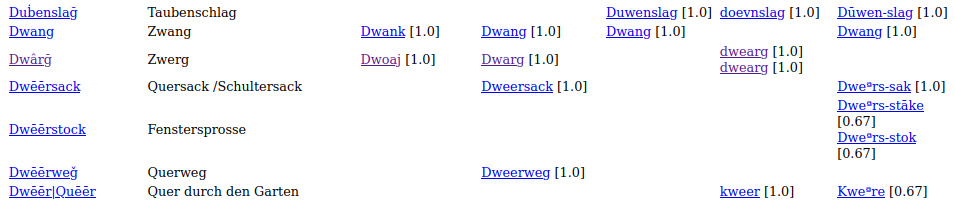
\includegraphics[width=1\linewidth]{img/html.png}
    \caption{Interdialectal link index, HTML export, columns from left to right: WöWö, German translation (WöWö), Plautdietsch, Plattmakers, Reuter, Twents, Westphalian}
    \label{fig-interdialectal-links-in-html}
\end{figure*}

\todo{update fig-interdialectal-links-in-html with Sass}

On this basis, we conducted a qualitative evaluation for 50 randomly sampled links predicted for WöWö and Plattmakers, and WöWö and the Westphalian dictionary, respectively, with results as summarized in Tab. \ref{tab-eval} and Fig. \ref{fig-eval}. 
Overall, we found the majority of links (82\% for Plattmakers, 64\% for WWB) to represent exact or approximative matches, and in line with relative proximity of Plattmakers and WöWö varieties, with much better results for Plattmakers. One major reason for the high number of mismatches is that North Low Saxon (WöWö and Plattmakers) normally drop unstressed Middle Low German e (apocope and syncope), whereas the Westphalian varieties (WWB and Twents) normally maintain it. 
As we cannot reliably distinguish stressed and unstressed syllables, the Westphalian (WWB and Twents) normalization allows to omit \emph{any} \word{e}, so that words like Twents \word{efn} `respectable' and \word{ven} `swampy meadow' include the same (possible) normalizations and can thus be easily confused. As we use Levenshtein distance as an additional disambiguating factor along with normalization-based confidence, dialects with apocope and syncope are likely to yield similar results, whereas the degree of variation (and the Levenshtein distance) is generally greater to dialects without apocope.

By approximative matches, we mean that either one of the words in a multi-word expression is identical, e.g., \word{Block Speck} `chunk of bacon' with Plattmakers \word{Block} `block, chunk, large piece', or that it involves a more or less transparent shift of meaning, e.g., \word{Ool} `eal' with Twents \word{Oal} (derogative nickname for persons notorious for speaking glibly), based on Twents \word{oal} `eal' (which is also linked). 
Aside from clearly incorrect links, the category of mismatches also includes homophones, e.g., WWB \word{Ō¹st} `branch' and \word{Ō²st} `east', which are historically unrelated, but formally identical (in some varieties, at least), and can thus not be disambiguated by any method of form-based matching.  We conclude that our formal linking method represents a reasonable baseline for future research to improve upon.
In particular, such improvements can be achieved if meaning relations (i.e., the glosses, definitions and translations in the respective dictionaries) are taken into account. 
For the time being, we recommend downstream applications for the cross-dialectal linking to operate with high-confidence links, only, i.e., cases in which the lack of ambiguity in the formal agreement indicates a reliable link. For the cautious user, we recommend a confidence threshold of $>0.5$, as this entails that at least one direction of the linking was formally unambiguous. 

\begin{table}
        \centering
        \begin{tabular}{lcc}
        & Plattmakers & WWB \\
        match & 33 & 29 \\
        approximative match & 8 & 3 \\
        mismatch & 9 & 18 \\
    \end{tabular}
    \caption{Qualitative evaluation over 50 WöWö links for Plattmakers and WWB dictionaries}
    \label{tab-eval}
\end{table}

\begin{figure}
    \centering
    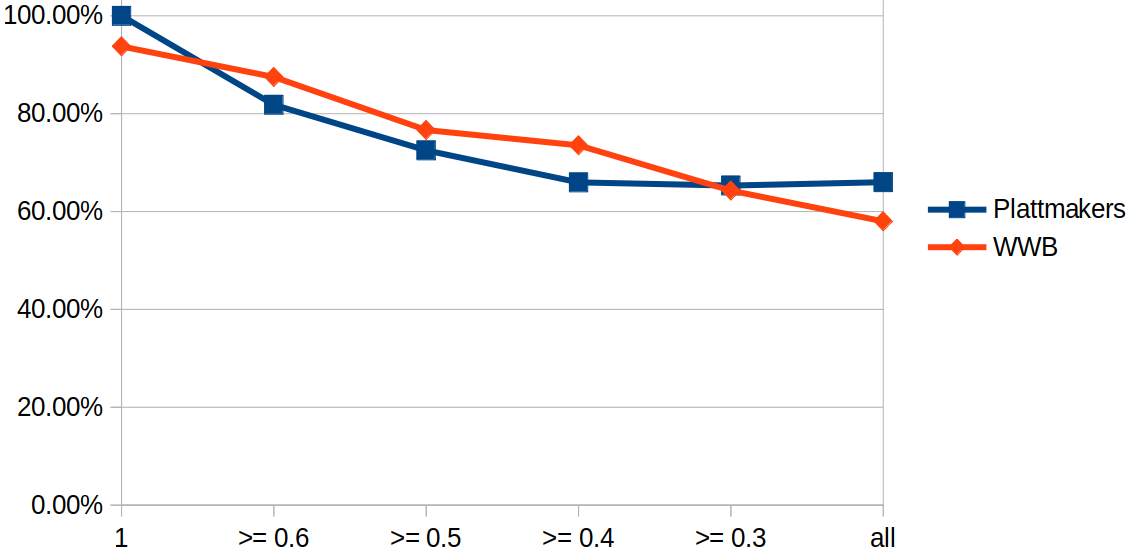
\includegraphics[width=0.5\linewidth]{img/confidence-vs-accurracy.png}
    \caption{Accuracy trade-off for 50 randomly sampled WöWö links with Plattmakers and WWB}
    \label{fig:enter-label}
\end{figure}

\begin{figure}
    \centering
    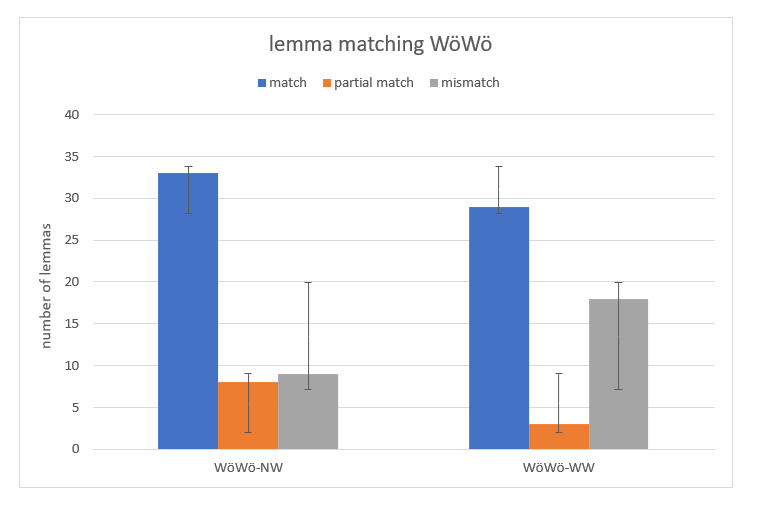
\includegraphics[width=1\linewidth]{lemma-matching-woewoe.png}
    \caption{Qualitative evaluation over 50 WöWö links for Plattmakers and WWB dictionaries}
    \label{fig-eval}
\end{figure}


The total number of links predicted for individual dictionaries is summarized in Tab. \ref{tab-results}, reporting only the most confident link for every source dictionary lemma.
In total, the linking covers 8,001 WöWö entries, thus conforming these to be lemma forms. This number appears to be small in comparison to the 26,713 of the WöWö in total, but to a large extent, this is due to compounds and derived forms that were included in WöWö, but not (or, at least, not as independent lemmas) in the other dictionaries. As such, we have 41 WöWö lemmas for \word{trecken} `to pull' and its derived forms in WöWö, but only 18 of these have been linked. The reason is not so much that words such as \word{rantrecken} `to pull here', \word{rintrecken} `to pull inside', \word{roptrecken} `to pull up there', \word{rövertrecken} `to pull over', \word{rumtrecken} `to pull over', or \word{ruuttrecken} `to pull out' don't exist in the other varieties, but they haven't necessarily been included in the other dictionaries because their formation follows a regular and productive morphological pattern and they don't convey a semantic meaning that cannot be deduced from its parts. In fact, any locative adverb can be combined with \word{trecken} and similar verbs of motion. The same holds true for nominal compounds, which are about as productive as in High German, but are normally not included in the other dictionaries unless they have special semantics that cannot be derived from its parts.

Furthermore, the WöWö contains a considerable number of phrasal expressions, which are not necessarily included in the other dictionaries, because these take a primary stance on documenting lexical semantics, not idiomatic expressions. The phrase \word{wat se wull, dat wull se} `what she wants, she wants' is an established idiom, but simply beyond the scope of word-centered (rather than collocation) dictionaries. Likewise, WöWö aims to be a practical tool for the modern day, and so it includes reference translations for certain institutions which are, however, just translated word by word from their respective national language. The \word{Zentroolroot vun de Juden} `Central Council of Jews (in Germany)' mirrors German \word{Zentralrat der Juden} almost exactly, except that the German genitive has been translated as a prepositional phrase. This is necessary because the genitive case was eliminated in North Low Saxon (and other dialects with apocope), this is informative for users of the dictionary (because it gives them a reference translation), and so, this is a legit entry. However, it can also be predicted by any competent speaker from the official designation in German. It is nevertheless a legit entry to the WöWö as a practical dictionary, because it helps its users to find appropriate expressions in cases in which there is a risk to resort to a High German loan construction (such as the genitive, in this case).

Beyond that, there are truly regional expressions or morphophonological processes. By comparison with its High German cognate \word{abgeordnet}, the WöWö term \word{afornt} `delegated' can be constructed to have underlying Low German reference form like \word{*av-ordņt}. But the consonant cluster \word{ordņt} may have been a bit of a challenge to speakers, and the WöWö entry indicates some simplification: The syllabic n has been simplified and the d has been assimilated with the r. Even though similar reduction processes exist in other dialects, as well, the specific result may be different, so that a direct 1:1 correspondence may not be found. Apocope and syncope are wide-spread phenomena in Low German, so that reduction and simplification processes are omnipresent, but with the lack of standard variety to orient towards since the demise of the Hanse, these processes produced regionally different results, and capturing them exhaustively with the FST approach pursued here would be intractable.

\section{Summary and Discussion}

We propose a method for creating a cross-dialectal lexical resource for Low German using LLOD technologies. This approach is particularly suited to a language that lacks a standardized written form, exhibits multiple conflicting orthographies, and shows significant internal variation in phonology, spelling, and grammar. 
We provide a conversion of the WöWö dictionary of the Dithmarschen dialect of North Low Saxon into RDF and use this as a lexical backbone. In a second processing step, this was enriched with cross-dialectal links based on formal agreement of WöWö lemmas with lexical entries from dictionaries of 6 other Low German dialects.
This data is provided as RDF data, with three files representing the original WöWö and one RDF file per external dictionaries. These RDF files define lexical entries and their respective canonical forms, but they do not provide additional details beyond the location of the corresponding lexical entry on the web -- the URI of the lexical entry is the URL of the underlying lemma. With the external dictionaries not providing an RDF view on their content, this is not actually linked data, as these URIs do not resolve to machine-readable data, but it is possible to query the graph and to provide a tabular export that not only includes (excerpts of) WöWö information, but also links with external dictionaries.

We provide an HTML view on this tabular export, and for a human, this HTML file (resp., for a machine, the underlying RDF data) is actually capable of serving as a ``digital Rosetta Stone'', linking dictionaries and mapping corresponding words across dialects -- without resorting to a standard variety or spelling (which, for the case of Low German, does not exist). 
% mögliche nutzung: es gibt keine dialektübergreifenden paralleltexte, aber mit verknüpften wörterbüchern könnte man multidialektale word embeddings (und, darauf aufbauend, multidialektale contextualized embeddings) induzieren. jeder der drei dialekte hat eine eigene literatur in unterschiedlichen orthographien.
Aside from supporting speakers and learners in their exploration of interdialectal differences and similarities, this approach also enables new applications in the technical realm: Since there are no cross-dialectal parallel texts for Low German, linking dictionaries could facilitate the induction of multidialectal word embeddings -- and, building upon that, multidialectal contextualized embeddings. Each of the dialects examined here has its own literary tradition, written in different orthographies.

% die daten können sich gegenseitig anreichern. wir haben definitionen und belege aus mehreren wörterbüchern. auch bei der phonologie: die vollwertige erfassung der phonologie erfordert, ein komplexes inventar von ê- und ô-Phonemen zu unterscheiden, die in keinem dialekt vollständig unterschieden werden, aber in ihrem zusammenwirken die verteilung von oo/au bzw. ee/ei in den unterschiedlichen dialekten erklären. auch bei der morphologie: nordniedersächsisch und mecklenburfisch sind apokopierend, westfälisch nicht, man bekommt also "ursprünglichere" Endungen und silben. das kann helfen, die phonologie zu klären, da "überlänge" oft nicht geschrieben wird. nochmal phonologie: plattmakers bietet IPA, alle anderen nur (mehr oder minder defektive) orthographien. dadurch ist eine disambiguierung der phonologie möglich.

Also, the data sources complement each other. We have definitions and attestations from multiple dictionaries. This applies to phonology as well: a comprehensive representation of phonology requires distinguishing a complex inventory of modern reflects of Middle Low German ê and ô phonemes (ê¹, ê², ê³; ô¹, ô², ô³; plus the umlaut forms of ô). 
In none of the dialects considered here, these are fully differentiated, but only collectively, they account for the distribution of resp. /e:/ $\sim$ /ɛɪ/ $\sim$ /aɪ/, /o:/ $\sim$ /ɔʊ/ $\sim$ /aʊ/, and /ø:/ $\sim$ /œʏ/ $\sim$ /ɔɪ/ in different modern dialects \cite{seelmann1908mundart}. Morphology, too, varies: Northern Low Saxon and Mecklenburgian exhibit apocope, whereas Westphalian does not, preserving ``original'' endings and syllables. If a Westphalian form is linked with a North Low Saxon form, this can aid phonological disambiguation, as apocope and syncope are compensated by lengthening of preceding vowels, but this is often not explicitly marked in writing (and in fact, this is a systematic shortcoming of all German-based orthographies of Low German). In addition, some external dictionaries actually provide phonological forms in IPA (esp., Plattmakers), and this can be exploited to compensate the shortcomings of the orthographic spelling conventions adopted and thus enables phonological disambiguation across dialects.

While the linking method employed here primarily serves to establish a baseline for future research, our cross-dialectal dictionary serves as a testbed for a number of community standards for machine-readable dictionaries on the web in general, and for non-standardized, low-resource languages in particular.
We observed a number of potential gaps in the existing OntoLex vocabularies. 

\begin{enumerate}
\item As our interdialectal links are created by heuristic means, we would like to be able to express to what extend a user can rely on the information conveyed by a link. This includes \emph{candidate links} (with a property such as `\onto{...:possibleMatch}'), but also the possibility to mark a link as an unverified (and eventually, as a verified) hypothesis.
\item More generally, it would be good to have a standard vocabulary for confidence in OntoLex, resp., LexInfo. Prov-O does not provide a codified vocabulary for expression confidence scores, in fact, the PROV-O documentation has an example that uses a \emph{local} property to provide that information. As a result, PROV-O applications have resorted to their own properties for this purpose, e.g., nif:taIdentConf, nif:taClassConf, or nif:confidence in the NLP Interchange Format (https://nif.readthedocs.io/en/latest/prov-and-conf.html). However, these properties are designed for a different purpose (linguistic annotation, esp., for named entity recognition and entity linking), and should not be applied to lexical linking. It should be noted that confidence scores are a recurring component of lexical resources, but apparently, no standard practice has been established in that regard (e.g., https://aclanthology.org/W19-5104.pdf actually provide examples with confidence scores in their source data, but seem to exclude them from the conversion, probably due to a lack of a standard vocabulary). At the same time, this is an intensely researched (yet, not satisfyingly solved problem) in the RDF world, and one of the key motivations driving the development of RDF-star.\footnote{\url{https://www.w3.org/groups/wg/rdf-star/}}
\item Lexinfo currently does not support the reification of \onto{lexinfo:geographicalVariant} (and its sibling properties). As we have to point with \onto{lexinfo:category} to an object property, we move the entire dataset out of the realm of OWL2/DL and into OWL2/Full. As a result, standard reasoning techniques cannot be applied to the resulting lexical knowledge graph. It would be ideal, if there would be an individual with a similar meaning.
\end{enumerate}

In addition to this, we found some solutions for apparent OntoLex gaps, but these may entail future simplifications of OntoLex.
As such, there is an apparent gap of a counterpart of translation sets for relations other than translations in OntoLex-VarTrans. 
However, introducing these for any kind of lexical-semantic relation would obfuscate the model. In fact, we did find a good work-around in \onto{dct:Dataset}, and we would suggest this as a best practice for other types of lexical-semantic relations, as well. Yet, to align this approach better with the current treatment of translation( set)s, we suggest to re-define \onto{vartrans:TranslationSet} as a subclass of \onto{dct:Dataset} (and \onto{vartrans:trans} as a subproperty of \onto{dct:hasPart}) and to motivate it as such in a future revision of the VarTrans module. This would be a backward-compatible revision that comes without any additional overhead (i.e. newly introduced concepts). A more radical alternative would be to deprecate \onto{vartrans:TranslationSet} and \onto{vartrans:trans} in favour of \onto{dct:Dataset} and \onto{dct:hasPart} (resp., its inverse, \onto{dct:isPartOf}.

Finally, a remark on language tags for Low German: 
The current ISO 639 language tags for Low German language varieties do not correspond to linguistically well-defined areas, but they involve a political dimension.
In particular, all regional dialects of Low German in the Netherlands have their own ISO 639-3 tag in addition to the ISO 639-2 tag \code{nds}, the `standard' tag for Low German is that alludes to the self-designation \word{Nedersaksisch} (in the Netherlands), resp., \word{Nedersassisch} (in Western parts of Germany; another self-designation is \word{Plattdüütsch}, which also is the preferred self-designation in some dialects, including the emmigrant variety of \word{Plautdietsch} that was, accordingly, assigned the ISO 639-3 language tag \code{pdt}). On the other hand, language tags for dialects outside the Netherlands are much less fine-grained, so that the six Dutch Westphalian dialects actually describe subsets of \code{wep} (for Westphalian). As a result, there is some confusion as to which varieties \code{nds} and \code{wep} actually refer to, and we see a lot of diversity in the use of language tags on the web. Even though ISO 639-3 \emph{seems} to restrict \code{nds} to Low German varieties in Germany (because all Dutch varieties of Low German have their own ISO 639-3 language tag), the largest collection of digital data of Low German from the Netherlands is actually designated by the BCP47 code \code{nds-nl}, i.e., `(German?) Low German in the Netherlands'.\footnote{\url{https://nds-nl.wikipedia.org}} 
With two `major' language tags applied to West Low German (\code{nds} and \code{wep}; plus \code{frs} for Low Saxon East Frisian), it has also become unclear how to properly identify East Low German. Glottolog.org resorted to redefine \code{nds} as `East Low German' and to address all non-Westphalian varieties of West Low German as \code{frs} -- although this is defined as `(Low Saxon) East Frisian'.\footnote{
  The tag \code{frs} was introduced for `East Frisian' in ISO 693-2, but defined there merely by a name list and without extensive documentation. Subsequently, ISO 693-3 assumed that this refers to Low Saxon East Frisian, and thus introduced a novel language tag \code{stq} for East Frisian proper (the Frisian dialect that was largely replaced by Low Saxon East Frisian), which was assumed to be lacking. However, linguistically, Low Saxon East Frisian is a variety of North Low Saxon and probably received this assignment by error, or by analogy with the main varieties of the Frisian (non-Low Saxon) language, \code{fry} (West Frisian) and \code{frr} (North Frisian).
} In the reality of the web, however, \code{nds} is used for Westphalian and North Low Saxon varieties of the Netherlands (e.g., in the Dutch Low German Wikipedia), as well as North Low Saxon in Germany (in the [German] Low German Wikipedia, written in accordance with Sass, i.e., \code{nds-x-hols1234} for Holstein North Low Saxon, albeit as an orthographic standard, not as a standard variety).\footnote{
    \url{https://nds.wikipedia.org/wiki/Wikipedia:Platt,_wo_schriev_ik_dat\%3F}
}
Here, we take \code{nds} to include all parts of North Low Saxon (in Germany) and Mecklenburg-Western Pomeranian, but to exclude Dutch Low German, Westphalian and Low Saxon East Frisian.\footnote{
  We make no claims about the use of language tags for varieties not covered in our sample of dictionaries, in particular, Eastphalian, North and Central Markian, Central Pomeranian, Eastern Pomeranian (extinct) and Low Prussian (extinct). Traditionally, Eastphalian, Westphalian and North Low Saxon (including the Dutch dialects) are grouped together as Western Low German, whereas Mecklenburgian, Pomeranian, Markian and Low Prussian varieties are grouped together as Eastern Low German.
}
However, this is problematic insofar as \code{nds} does not refer to a linguistically well-defined group of dialects, and we would like to encourage future discussions on revising the ISO 639-3 language tags, accordingly.

Overall, we succeeded in creating our `Rosetta stone' for almost the entirety of Low German in the sense that there now is a human- and machine-readable lexical knowledge graph of (North Low Saxon) lemmas and their interdialectal links into other, externally hosted dictionaries.
However, while we were using standard LLOD technologies to implement this interdialectal linking, we did not actually provide Linguistic Linked Open Data. Our WöWö data is linked with dictionaries in HTML, but not RDF -- with a notable exception being Plattmakers, which contains JSON-LD metadata. 
Furthermore, most of these linked data sources (including Plattmakers) are not actually `open' in the sense of the Open Definition. 
But our work represents a first step towards putting Low German on the map of Linguistic Linked Open Data, and a proof-of-principle of its capabilities.
In fact, it is a pity that LOD technology is not more widely supported by Wörterbuchnetz and DWN, as these are supported by researchers working in the field, and as they are actually designed to provide inter-dictionary links, although only \emph{within their own platform}. 
However, we hope that we've been able to demonstrate the added value of inter-dictionary links for Low German, and this solution organically extends to any other dictionary available via DWN or Wörterbuchnetz. Also, with technologies such as JSON-LD and RDFa, both these portals can actually be easily extended to provide LOD support on their own -- and to the best we can tell with minimal changes to their current workflows.
A future direction may thus be to encourage or to support the colleagues to integrate RDF technologies, and then, to really create an interdialectal, distributed meta-dictionary of Low German, and to facilitate the development of technologies and resources that benefit \emph{all} its varieties in their entirety.

% \subsection{Appendices}
% 
% Use \verb|\appendix| before any appendix section to switch the section numbering over to letters. See Appendix~\ref{sec:appendix} for an example.
%
%\section{Bib\TeX{} Files}
%\label{sec:bibtex}
%
%Unicode cannot be used in Bib\TeX{} entries, and some ways of typing special characters can disrupt Bib\TeX's alphabetization. The recommended way of typing special characters is shown in Table~\ref{tab:accents}.
%
%Please ensure that Bib\TeX{} records contain DOIs or URLs when possible, and for all the ACL materials that you reference.
%Use the \verb|doi| field for DOIs and the \verb|url| field for URLs.
%If a Bib\TeX{} entry has a URL or DOI field, the paper title in the references section will appear as a hyperlink to the paper, using the hyperref \LaTeX{} package.

\section*{Limitations}

% Since December 2023, a "Limitations" section has been required for all papers submitted to ACL Rolling Review (ARR). This section should be placed at the end of the paper, before the references. The "Limitations" section (along with, optionally, a section for ethical considerations) may be up to one page and will not count toward the final page limit. Note that these files may be used by venues that do not rely on ARR so it is recommended to verify the requirement of a "Limitations" section and other criteria with the venue in question.

The WöWö dictionary considered here is extremely rich and extremely dense in lexiographic and linguistic information, but this is provided in a semistructured format tailored towards human readers. As a result, it is virtually impossible to provide an exhaustive RDF formalization of its content. Instead, we extracted core aspects and demonstrated how these can be extended to include references to other dictionaries that may provide additional information, e.g., examples or (region-specific) definitions.

There are some limitations to our approach of linking. In particular, we excluded interlingual links, resp., additional translations, provided by the indexed dictionaries because of copyright considerations. Neither was part-pof-speech information included. Instead, we provide a purely form-based linking. While this may be further explored (both in its legal dimension and technical applications) in the future, the aim of the current paper is to develop a proof-of-principle implementation for an LLOD-based interdialectal lexical resource for the major dialects of Modern Low German, based on linking existing lexical resources accessible over the web with an RDF conversion of a North Low Saxon dictionary (WöWö). Specific challenges encountered include the complexity of the WöWö dictionary layout, legal constraints regarding the re-usability of external resources linked and aspects of data modelling. Interdialectal linking is solely predicted on grounds of formal agreement, without taking sense information or translations into account.

The primary concern of the paper is technical in nature, with a focus on normalizing divergent orthographies and phonological differences on the one hand, and on modelling issues on the other. We did not systematically assess the linguistic quality of the different dictionaries nor did we evaluate the quality of the generated links. 

In the absence of training data for interlingual mapping, we implement a linguistically informed normalization by means of traditional symbolic methods, and generate candidate matches between normalized source language lemmas and normalized WöWö lemmas, ranked by a confidence score that captures the level of (formal) ambiguity in n:m mappings. While the phonological correspondences are well understood and uncontroversial, this employs solely formal criteria, and is prone to link formally similar but semantically unrelated lemmas. This can be addressed in the future in different ways, e.g., by comparing translations and definitions provided by different dictionaries. This can be implemented by different techniques, including neural methods or lexical linking of existing lexical resources for German, Dutch and English (the primary languages of definitions), but is left as a topic for future research. 

% Bibliography entries for the entire Anthology, followed by custom entries
%\bibliography{anthology,custom}
% Custom bibliography entries only
\bibliography{bib.bib}

%\appendix
%
%\section{Example Appendix}
%\label{sec:appendix}
%
%This is an appendix.

\end{document}
